\documentclass[12pt]{article}
\usepackage{anyfontsize}
\usepackage[a4paper, margin=2cm]{geometry}
\usepackage{polski}
\usepackage{tabto}
\usepackage{enumitem}
\usepackage{amsmath}
\usepackage{multirow}
\usepackage{multicol}
\usepackage{setspace}


\usepackage{hyperref}
\hypersetup{
    colorlinks = true,
    urlcolor=blue
}

\usepackage{graphicx}
\graphicspath{{../Img/}}

\usepackage{titlesec}
\titlelabel{\thetitle.\quad}
% \AddToHook{cmd/section/before}{\clearpage}

\renewcommand{\figurename}{Zdjęcie}

\title{Propozycja projektu\\ \textbf{Robotyczne ramie} {\small \\ z przedmiotu: techniki mikroprocesorowe}}
\author{Łukasz Przystupa, Piotr Kowol}
\date{\today}

\usepackage{titling}
\renewcommand\maketitlehooka{\null\mbox{}\vfill}
\renewcommand\maketitlehookd{\vfill\null}

\begin{document}
    \begin{titlepage}
        \maketitle
        \thispagestyle{empty}
        \begin{center}
            Opiekun projektu: Sebastian Koryciak.
        \end{center}
    \end{titlepage}

    \section{Opis projektu}
        \tab Celem projektu jest zbudowanie oraz zaprogramowanie, robotycznego ramienia. 
        Sterowaniem zajmie się mikroprocesor RP2040 (Cortex M0+) z modułem Wi-Fi cyw43.
        Projekt zakłada dwu-wątkową aplikację napisaną w językach: C oraz JS.
        Program napisany w C będzie zawierał algorytmy sterowania, na przykład przetwarzanie wartości kartezjańskich na odpowiednie kąty dla serwomechanizmów.
        Natomiast część zbudowana w JS z pomocą HTML'a oraz CSS'a będą stanowiły interface użytkownika, pozwalający na swobodne kontrolowanie ramienia w wszystkich stopniach swobody.

    \section{Model ramienia}
        \tab Model ramienia jest otwarto źródłowym projektem udostępnionym na stronie \href{https://www.thingiverse.com/thing:1015238}{thingiverse.com}
        \begin{figure}[!ht]
            \centering
            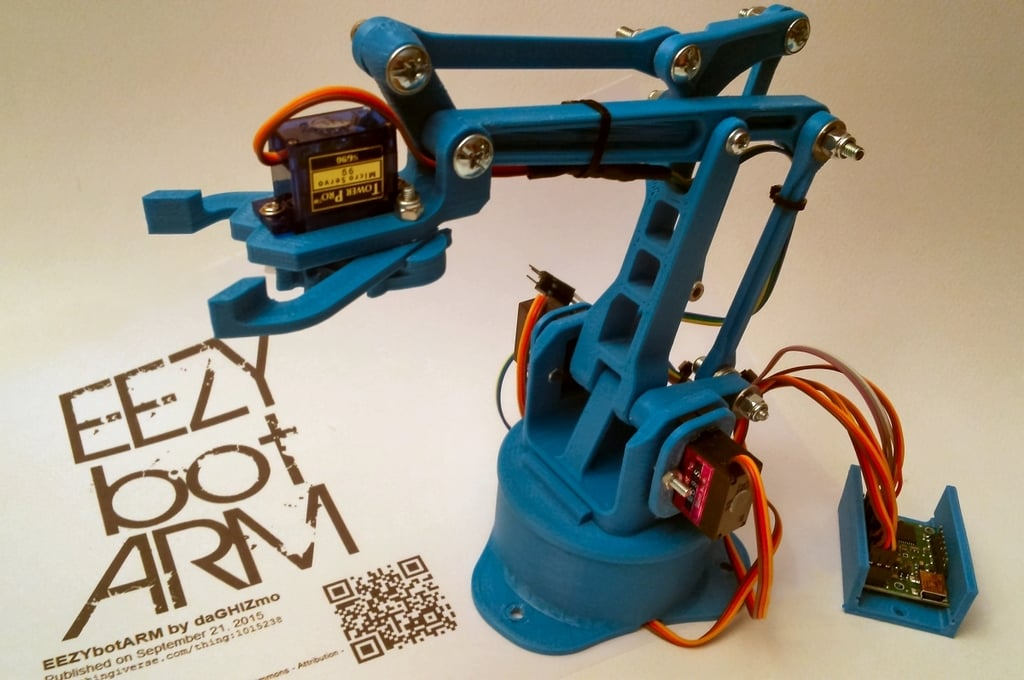
\includegraphics[width = 0.8\textwidth]{arm.jpg}
            \caption{Zdjęcie poglądowe z strony autora}
        \end{figure}\\
        Autor w projekcie zastosował „droższe” serwomechanizmy, jednak ze względu na dostępny budżet
         oraz możliwą kompatybilność wszystkie serwa w projekcie będą tanimi SG90.

    \section{Cechy dodatkowe}
        \begin{enumerate}
            \item Ze względu na dużą uniwersalność ramienia, silniki serwomechanizmów zostaną zabezpieczone zarówno hardwarewo
            jak i z pomocą softwaru.
            \begin{itemize}
                \item Zabezpieczeniem hardware będą wzmacniacze operacyjne z niewielkimi rezystorami w torze zasilania silników, 
                których zadaniem będzie pomiar prądu i w przypadku przekroczenia wartości krytycznej przez dłuższy czas odetną sterowanie układu.
                \item Zabezpieczenie software będzie polegać na pomiarze sygnału feedback serwa
                oraz w~przypadku braku zmian odcięcie sterowania silnika.
            \end{itemize}
            \item Dodatkowo zostanie napisana prosta symulacja działania ramienia w języku python w celu znalezienia najbardziej optymalnej funkcji przeliczania wartości z układu kartezjańskiego na wartości kątowe.
        \end{enumerate}

\end{document}